\newpage
\chapter{Trade-Off}
\label{ch-tradeoff}

%STICK TO THE STRUCTURE THAT IS INDICATED TO ENSURE CONSISTENCY, WE WILL BE WRITING THIS CHAPTER WITH MANY PEOPLE 

In this chapter, an overview of the trade off of concepts will be presented. Firstly, a set of concepts in three different passenger range categories will be created. A preliminary trade off of these concepts using only the quantitative parameters will be performed, in order to choose a winning concept from each passenger range that will enter the final trade-off. For this, the tool will be used to compute some useful outputs. The final trade-off, that follows after that, will then evaluate the full set of quantitative and qualitative parameters of the concepts, in order to choose the winning concept. In the final trade-off use will be made of the trade criteria defined in \autoref{CriteriaTools}, including the weighting factors found previously. 

\section{Design Definitions}
In order to evaluate each design concept using the tools, some basic parameters including MTOW, cruise speed, range and OEW/MTOW ratio, must be determined. Since many concepts are novel, they are compared to existing vehicles to determine if the combination of parameters are realistic. In \autoref{fig:MTOW-Pax2} and \autoref{fig:Cruise-MTOW2}, the same statistical plots from \autoref{stats} are given with the concepts included as light-blue diamonds. In the case of MTOW and cruise speed, they fall within realistic margins as shown in \autoref{fig:MTOW-Pax2} and \autoref{fig:Cruise-MTOW2} respectively. The range of many of the concepts was reduced from the maximum available, which results in lower battery mass. This accounts for some difference from statistics, but still results in a feasible design. This is done to better suit the market needs.

\begin{figure}[H]
\begin{subfigure}[t]{0.5\textwidth}
    \centering
    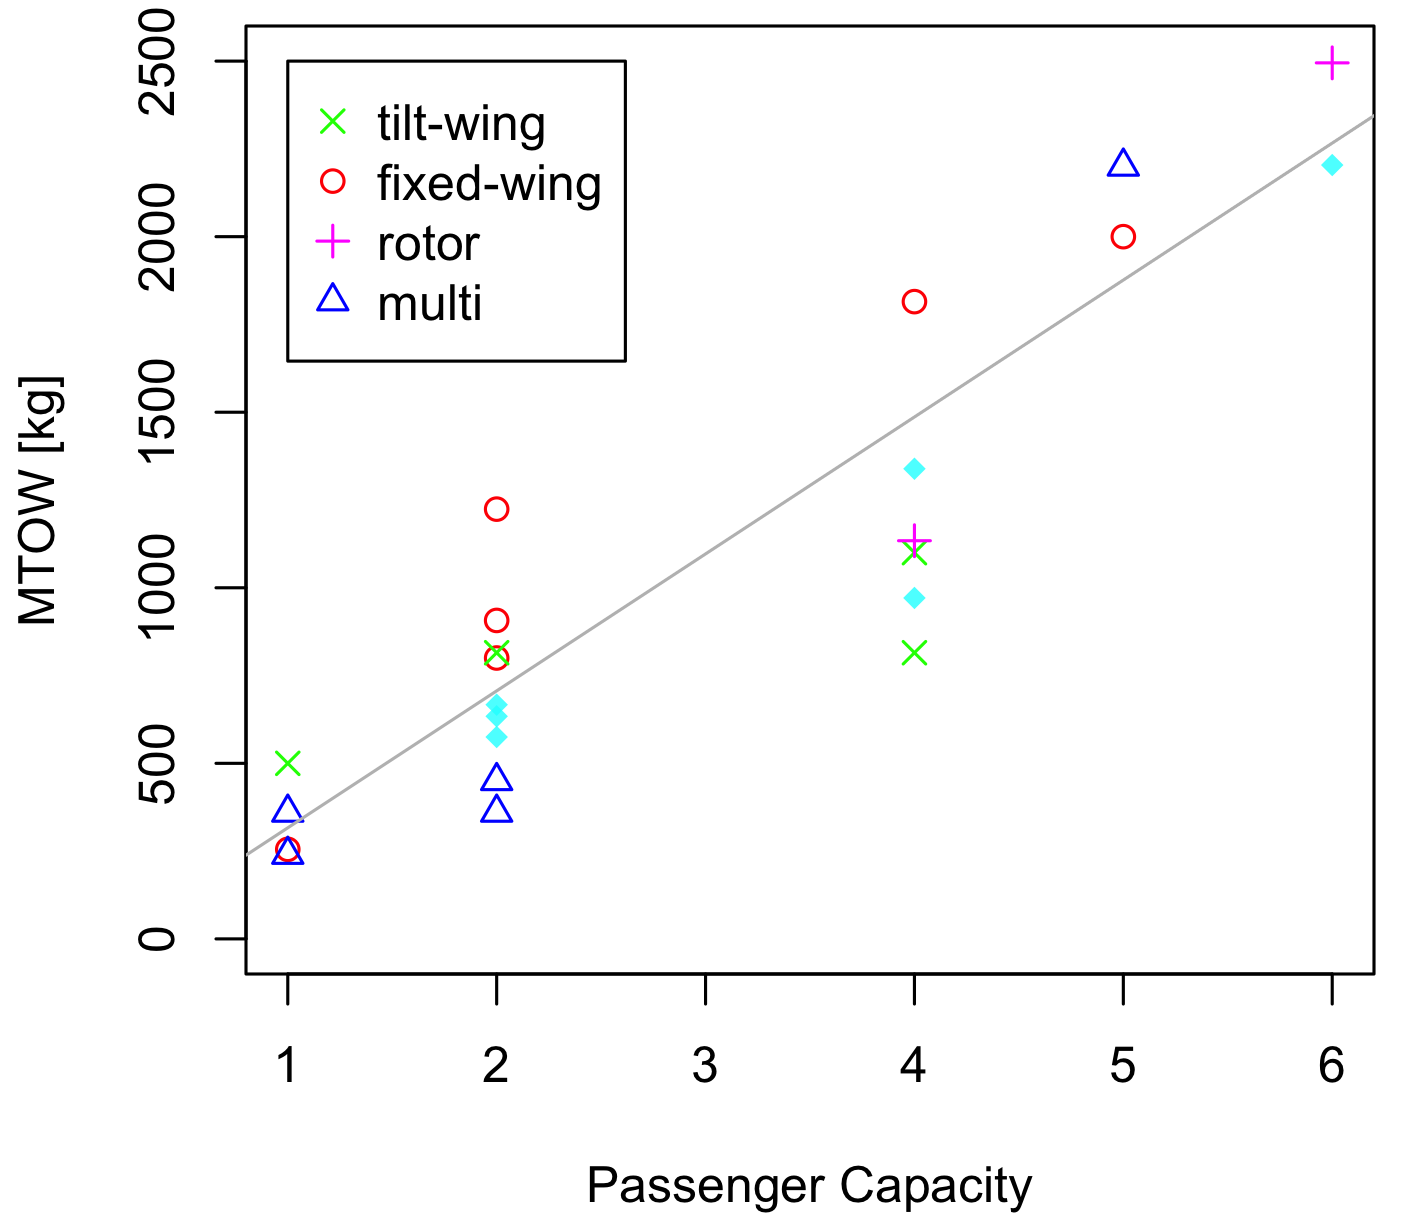
\includegraphics[width=\textwidth]{Figures/MTOW-Pax2.png}
    \captionsetup{width=.8\linewidth}
    \caption{When comparing MTOW to number of passengers, the designed concepts (blue diamonds) fit with existing statistics.}
    \label{fig:MTOW-Pax2}
\end{subfigure}
\begin{subfigure}[t]{0.5\textwidth}
    \centering
    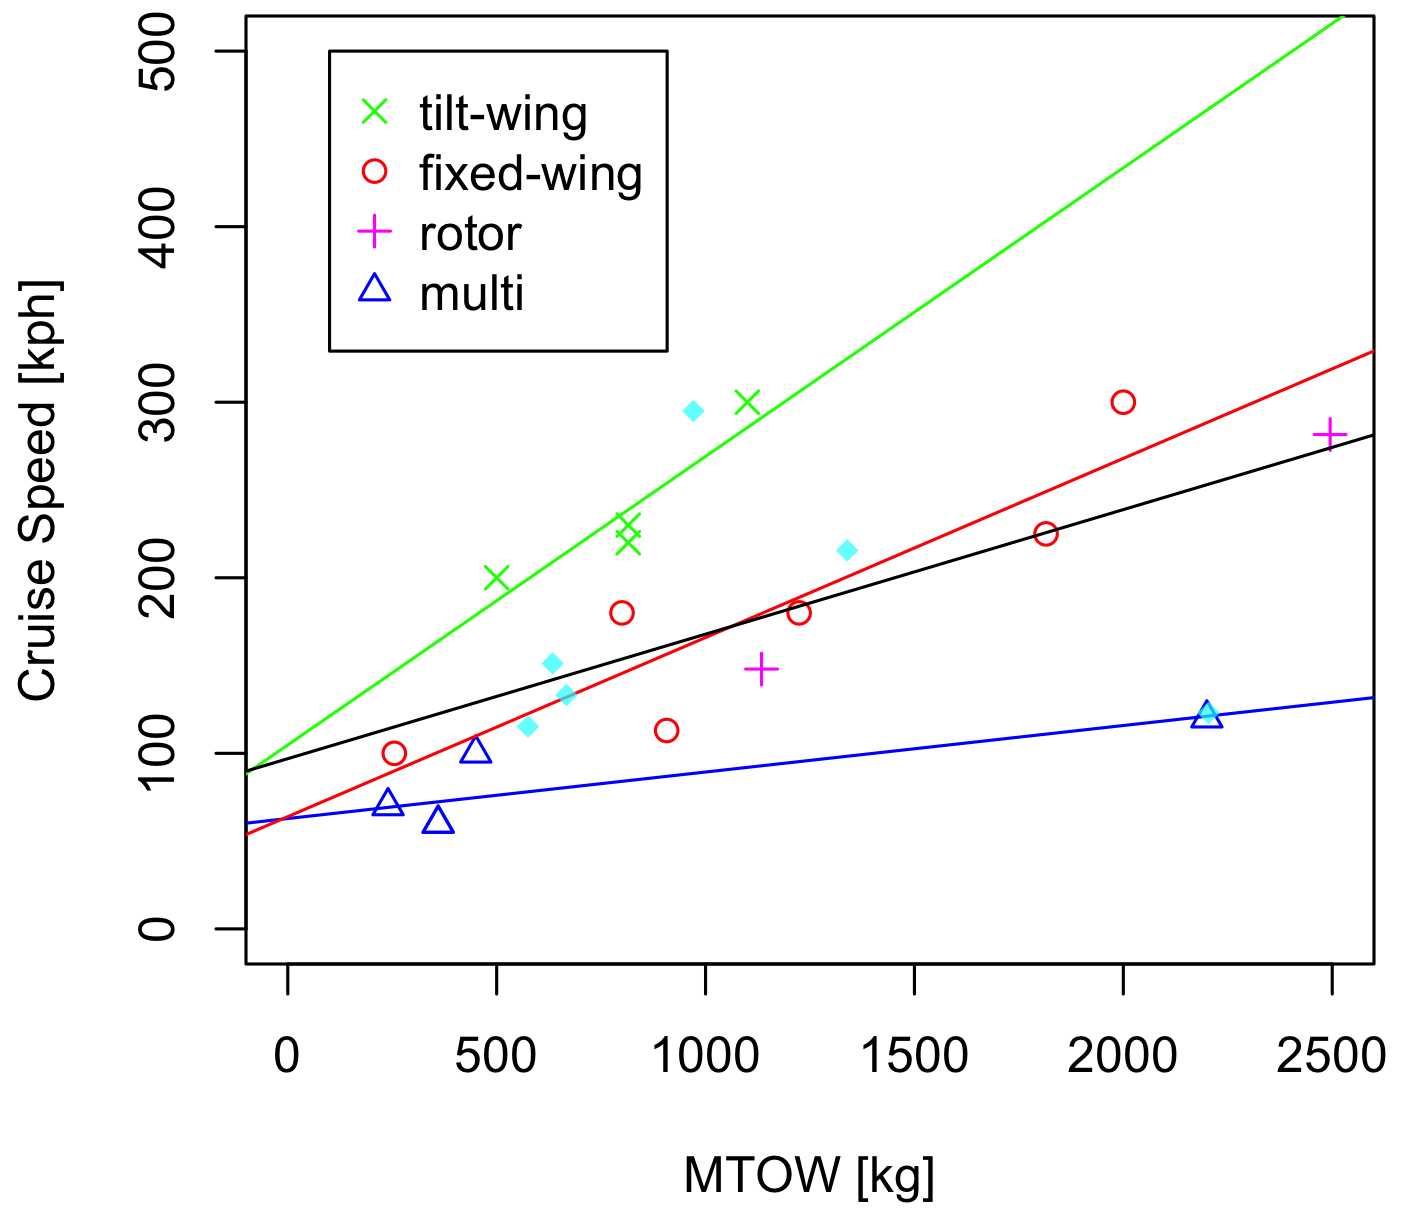
\includegraphics[width=\textwidth]{Figures/Cruise-MTOW2.png}
    \captionsetup{width=.8\linewidth}
    \caption{When comparing MTOW to cruise speed, the designed concepts (blue diamonds) fit with existing statistics.}
    \label{fig:Cruise-MTOW2}
\end{subfigure}
\label{fig:concept_compare}
\end{figure}

\section{1-2 Passenger Vehicles}
%Give a little introduction to 1-2 passenger vehicles 
A broad range of 1-2 passenger air vehicles has already been designed and thought of. However, most of these design are not commercially feasible, for example due to the fact that they are unsafe, aesthetically unpleasing or the choice of material is not sustainable. While brainstorming, the commercial feasibility of the design options was taken into account. Three concepts were thought of. The drawings of these concepts are presented in \autoref{1-2A}, \autoref{1-2B} and \autoref{1-2C}. The concepts are evaluated by using the integrated tool which was introduced in \autoref{sec:Tools}. The main parameters that were used as inputs are tabulated in \autoref{12input}. The resulting main outputs are presented in \autoref{12output}. 

\subsection{Concept Definition}
%Include figures and descriptions of vehicles, plus parameters that will go into the tool 

\begin{figure}[H]
  \centering
  \begin{minipage}[b]{0.25\textwidth}
    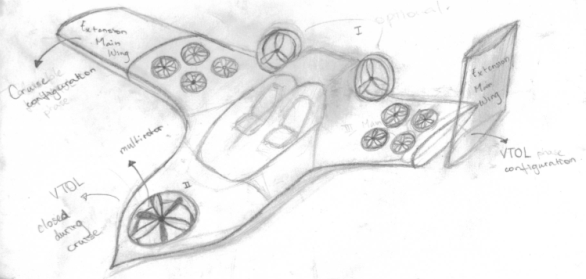
\includegraphics[width=5.0cm]{./Figures/Concept12a.png}
    \captionsetup{justification=centering}
    \caption{Concept 1}
    \label{1-2A}
  \end{minipage}
  \hspace{1.5cm}
  \begin{minipage}[b]{0.30\textwidth}
    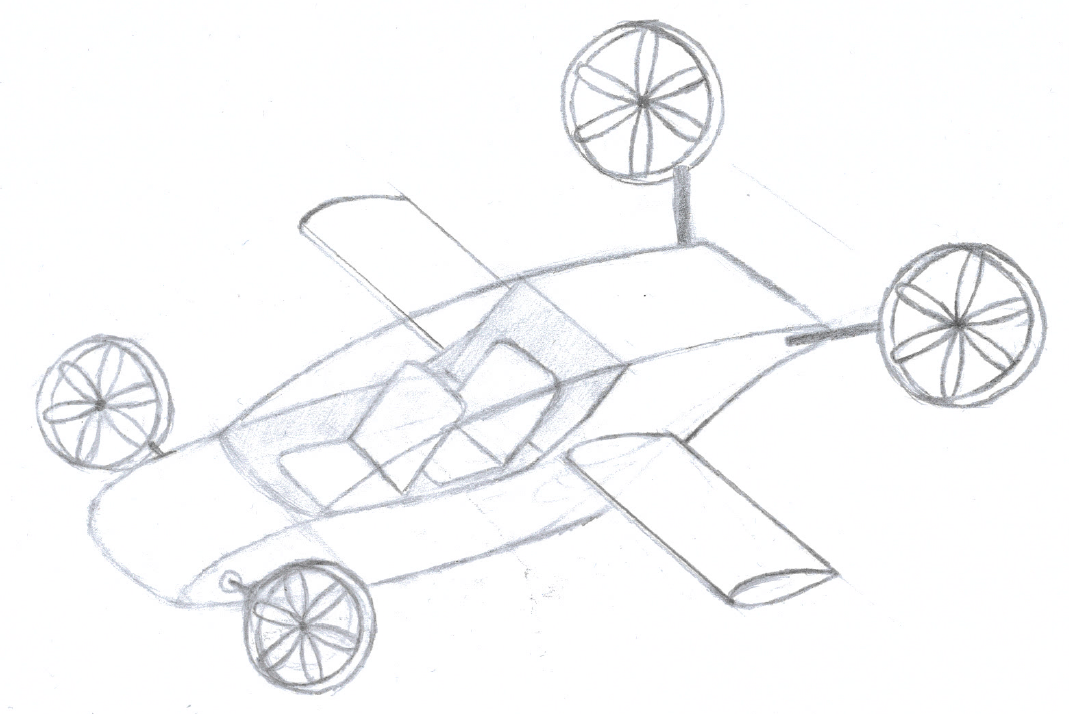
\includegraphics[width=5.0cm]{./Figures/Concept12b.PNG}
    \captionsetup{justification=centering}
    \caption{Concept 2}
    \label{1-2B}
  \end{minipage}
  \hspace{0.5cm}
  \begin{minipage}[b]{0.25\textwidth}
    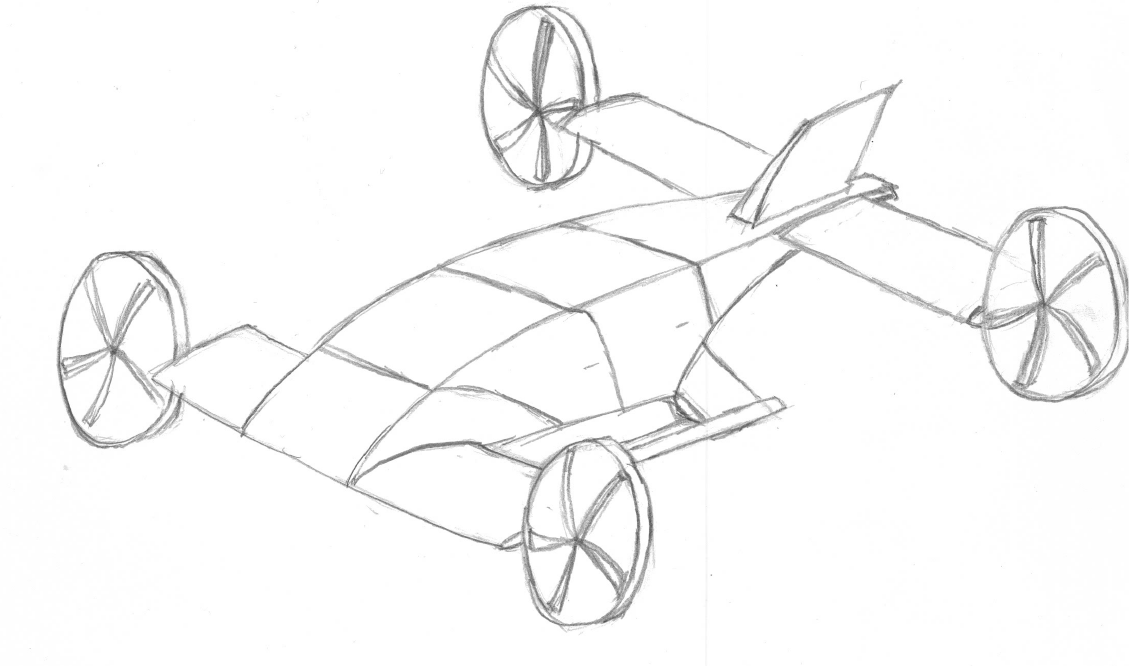
\includegraphics[width=5.0cm]{./Figures/Concept12c.PNG}
    \captionsetup{justification=centering}
    \caption{Concept 3}
    \label{1-2C}
  \end{minipage}  
\end{figure}

\paragraph{Concept 1}
Concept 1 is in essence a flying wing with a fan located in front of the cockpit, a set of fans located in the wing and a set of fans located in top of the wing next to the fuselage as seen in \autoref{1-2A}. The fan located in the front is a coaxial ducted fan which is solely used for vertical take-off and landing, and the latches are closed in the cruise configuration. The set of fans located in the wing are used for vertical take-off and landing, and are rotated $90\degree$ for the cruise configuration to produce thrust. One should acknowledge that the fans as seen in \autoref{1-2A} do not represent the final vehicle concept, as only one (bigger) fan is located per half span of the wing, rather than 4 per half span. The fans located on top of the wing rotate around the trailing edge of the wing and are fully horizontal in vertical take-off and landing configuration, and are used to produce thrust during cruise, as seen in the configuration shown in \autoref{1-2A}. Furthermore, the passenger seating arrangement is side-by-side and the passengers will enter the vehicle from the sides.

\paragraph{Concept 2}
The body of this particular concept has some resemblance with the shape of an airfoil. This way the body naturally produces lift by itself. In addition to this, a wing was added to increase the cruise performance. Furthermore, it has four tiltable rotors. The two rotors in the back have a slightly larger diameter than the rotors in the front. They are bigger, because it is expected that the center of gravity will lie somewhat aft. So by increasing their size, these rotors will be able to take up more of the required hover power enabling vertical take off without hanging to one side. Moreover, the two passengers are seated behind each other and will be able to enter the vehicle from the side. 

\paragraph{Concept 3}
The configuration of concept 3 is composed of front and rear wing surfaces, with tilt rotors at the tips of all the wing surfaces. These rotors therefore tilt horizontally to provide hover propulsion, which is when they are used at their maximum power output. During cruise, all rotors tilt vertically to provide horizontal propulsion, with the wing surfaces providing lift force to the vehicle. The rotors measure approximately 1.7 meters in diameter, making them relatively large and therefore making the total width consequentially large, and therefore space demanding. This also induces large tip loads on the wing structure which will require lots of structural reinforcement efforts. The seating configuration is a row of two seats, which satisfies the width minimisation required due to the already large wingspan due to large tip rotors and wing surfaces. The users would enter the vehicle from the side with doors placed on the side that open vertically.  

% iPce. elease add the foe vehllowing required packages to your document preamble:
% \usepackage{booktabs}
\begin{table}[H]
\captionsetup{justification=centering}
\caption{Input of tools for 1-2 person vehicle}
\label{12input}
\begin{tabular}{@{}llll@{}}
\toprule
\textbf{Parameter}                       & \textbf{Concept 1} & \textbf{Concept 2} & \textbf{Concept 3} \\ \midrule
MTOW {[}kg{]}                            &           634         &        575           &         667           \\
OEW/MTOW           &          0.45          &         0.40          &             0.47       \\
\# Passengers {[}-{]}                    &          2          &         2           &             2       \\
Range {[}km{]}                           &          60          &         60     &            60        \\
Max Dimension {[}m{]}                    &         5.75           &          5          &            6        \\
Battery Energy density {[}Wh/kg{]}       &           260         &       260  &            260        \\
Battery Power density {[}W/kg{]}         &           2100         &      2100 &            2100        \\
L/D {[}-{]}                              &           17         &        12            &           16         \\
Radius of rotors (x number of rotors) &   0.75 (1x) \& 0.4 (2x) \& 0.5 (2x)                &    0.85 (2x) \& 0.8 (2x)&            0.85 (x4)       \\
Cruise Velocity {[}m/s{]}                &          42          &        32            &            37        \\ \bottomrule
\end{tabular}

\end{table}


\subsection{Intermediate Trade-off}
%Present the outputs of the tools for each option, put it in a table and discuss which 1 (or 2) is best. Explain that we will continue with that one to the final trade off, where we will investigate that option further by looking at additional qualitative factors like user experience, passenger comfort, safety etc..   

The inputs that were mentioned in the previous section were put in a tool. The main results are tabulated in \autoref{12output}.

\begin{table}[H]
\captionsetup{justification=centering}
\caption{Output of tools for 1-2 person vehicle}
\label{12output}
\begin{tabular}{@{}llll@{}}
\toprule
\textbf{Parameter}                           & \textbf{Concept 2A} & \textbf{Concept 2B} & \textbf{Concept 2C} \\ \midrule
\# Vehicles {[}-{]}                          &         9800          &        12900        &           11200         \\
\# Pads {[}-{]}                               &       1570           &    1620      &  1610  \\
\# Trips/day {[}-{]}                         &          283000          &     308000          &           294000         \\
\#  PREE {[}Wh/(pax-km){]}           &          910          &       790     &        915      \\
\# Ticket price {[}\$/km{]}                  & 2.86                   & 2.34                   & 3.04                    \\
\# Ticket price {[}\$/km-pad costs{]}        & 0.64                    & 0.62                   & 0.65                   \\
\# Passengers/day {[}-{]}                    &          30500          &     32700        &           31400        \\
Vertiport Area {[}m\textsuperscript{2}{]}    &          760          &      630        &           830      \\
Total System Area {[}km\textsuperscript{2}{]} &          1.19         &     1.01  &         1.34         \\
Total Board Time {[}s{]}                     &          210          &     210               &               210     \\
Noise {[}dBA{]}                              &             82       &     71          &           73        \\
Downwash {[}m/s{]}                              &             51       &     34          &           36        \\ \bottomrule
\end{tabular}
\end{table}

After comparing the results shown in the table above, concept 2 was chosen as the winning concept for this particular vehicle capacity. This concept scored best in terms of energy usage, ticket price per km, size of the vertiport area, total system area and noise level. Concept 3 had the lowest amount of vehicles and pads, but it also served a fewer amount of trips and passengers per day. So these somewhat better results do not outweigh all the results on which concept 2 scores better. Concept 1 is omitted, since the noise level is too high, an excessive amount of vehicles is required and the ticket price per km is quite high. Moreover, concept 2 seems to be the most sustainable during operation due to the low energy usage. Concept 2 will be worked out in greater detail in \autoref{Sec:FinalTO}. 



\section{4-6 Passenger Vehicles}
%Give a little introduction to 4-6 passenger vehicles 
The range of 4-6 passengers is an interesting market for the urban air mobility. It has the experience of a taxi in the air. Lately, Lilium launched their five passenger vehicle \footnote{\url{https://lilium.com/the-jet} [accessed 21-05-19]}. 


At the end of the section, one 'winner' will be selected to investigate further and compare to the best concepts for the other vehicle capacities. 

\subsection{Concept Definition}
%Include figures and descriptions of vehicles, plus parameters that will go into the tool. 
Based on research of existing air taxi concepts, the majority of well-developed vehicles fall into 3 categories. As an initial trade-off, one vehicle from each of these categories is considered. In each case, the OEW/MTOW (not including the battery mass) is set at a specific ratio. This is done to prevent unrealistic designs. The effect of this choice will be considered in the sensitivity analysis. During the design process for the 4-6 vehicles, different sensitivity analysis were done e to come up with the best capacity for each vehicle. Next to that, the speed and range are adjusted during the design phase to find the optimal parameters. 

\paragraph{Concept 1: The Electric Jet}
The first vehicle considered is called the "Electric Jet" (\autoref{4-6A}), and is similar to the Lilium Jet\footnote{\url{https://www.lilium.com} [accessed 21-05-19]}. It features fixed wings in a canard configuration. Along the wings are smaller electric turbines. While this vehicle is designed for highly efficient and low-drag forward flight, it also has very high disk loading in hover and takeoff. During market analysis, there is little demand for long duration journeys, so a scaled 4 passenger version is presented for trade-off. The passengers sit 2x2 and board from both sides.

\paragraph{Concept 2: The Tilt-Wing}
Another concept category is the Tilt-wing, as depicted in \autoref{4-6B}. This concept has 4 large propellers mounted on forward swept tilt-wings. When the wings tilt up for takeoff and landing, the rotors raise up, and provide safe clearance. A canard wing and nose rotors are also needed for balance in hover. A pusher fan (or two) are also attached at the stern for use in forward flight. From the statistics, winged aircraft gain significant efficiency advantage in forward flight, and also can attain higher speeds. The passengers sit 2x2 and board from one side. This concept will allow for a bit more forward space than the electric jet in order to accommodate boarding.

\paragraph{Concept 3: The Gondola}
In \autoref{4-6C} a vehicle design for six passengers can be seen. The vehicle looks like a gondola. There are two benches in the vehicle where three people can sit on each bench. On top of the vehicle 4 coaxial rotors are placed. They will be placed outwards of the vehicle to make sure that the rotors will produce a better lift. Next to that, the rotors should be placed as much as possible outwards to prevent the interference of noise with the vehicle. On the bottom the landing gear of the vehicle is placed. The landing gear is designed as a box within a wheel, this is useful for taxiing. These constructions are placed on each corner of the vehicle. As can be seen in the figure there is room under the benches to store the batteries. 
\begin{figure}[H]
  \centering
  \begin{minipage}[b]{0.25\textwidth}
    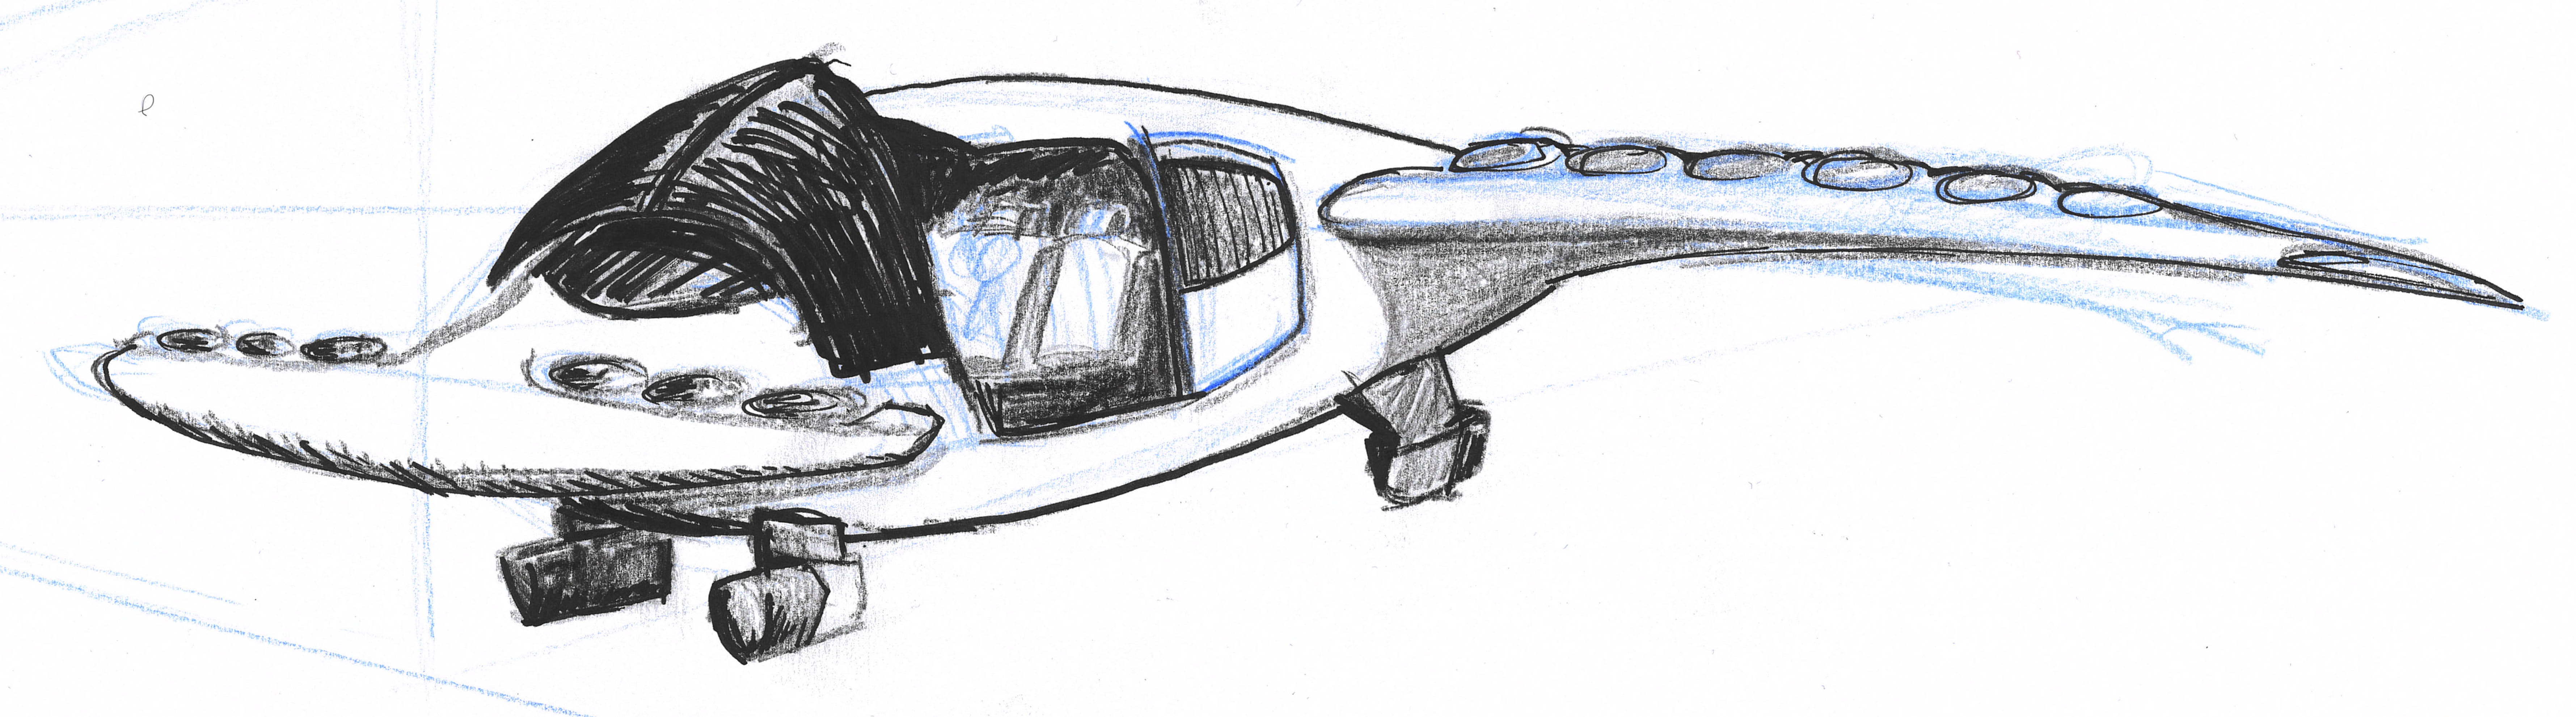
\includegraphics[width=5.0cm]{./Figures/ejet.jpg}
    \captionsetup{justification=centering}
    \caption{Electric Jet 4}
    \label{4-6A}
  \end{minipage}
  \hspace{1.5cm}
  \begin{minipage}[b]{0.30\textwidth}
    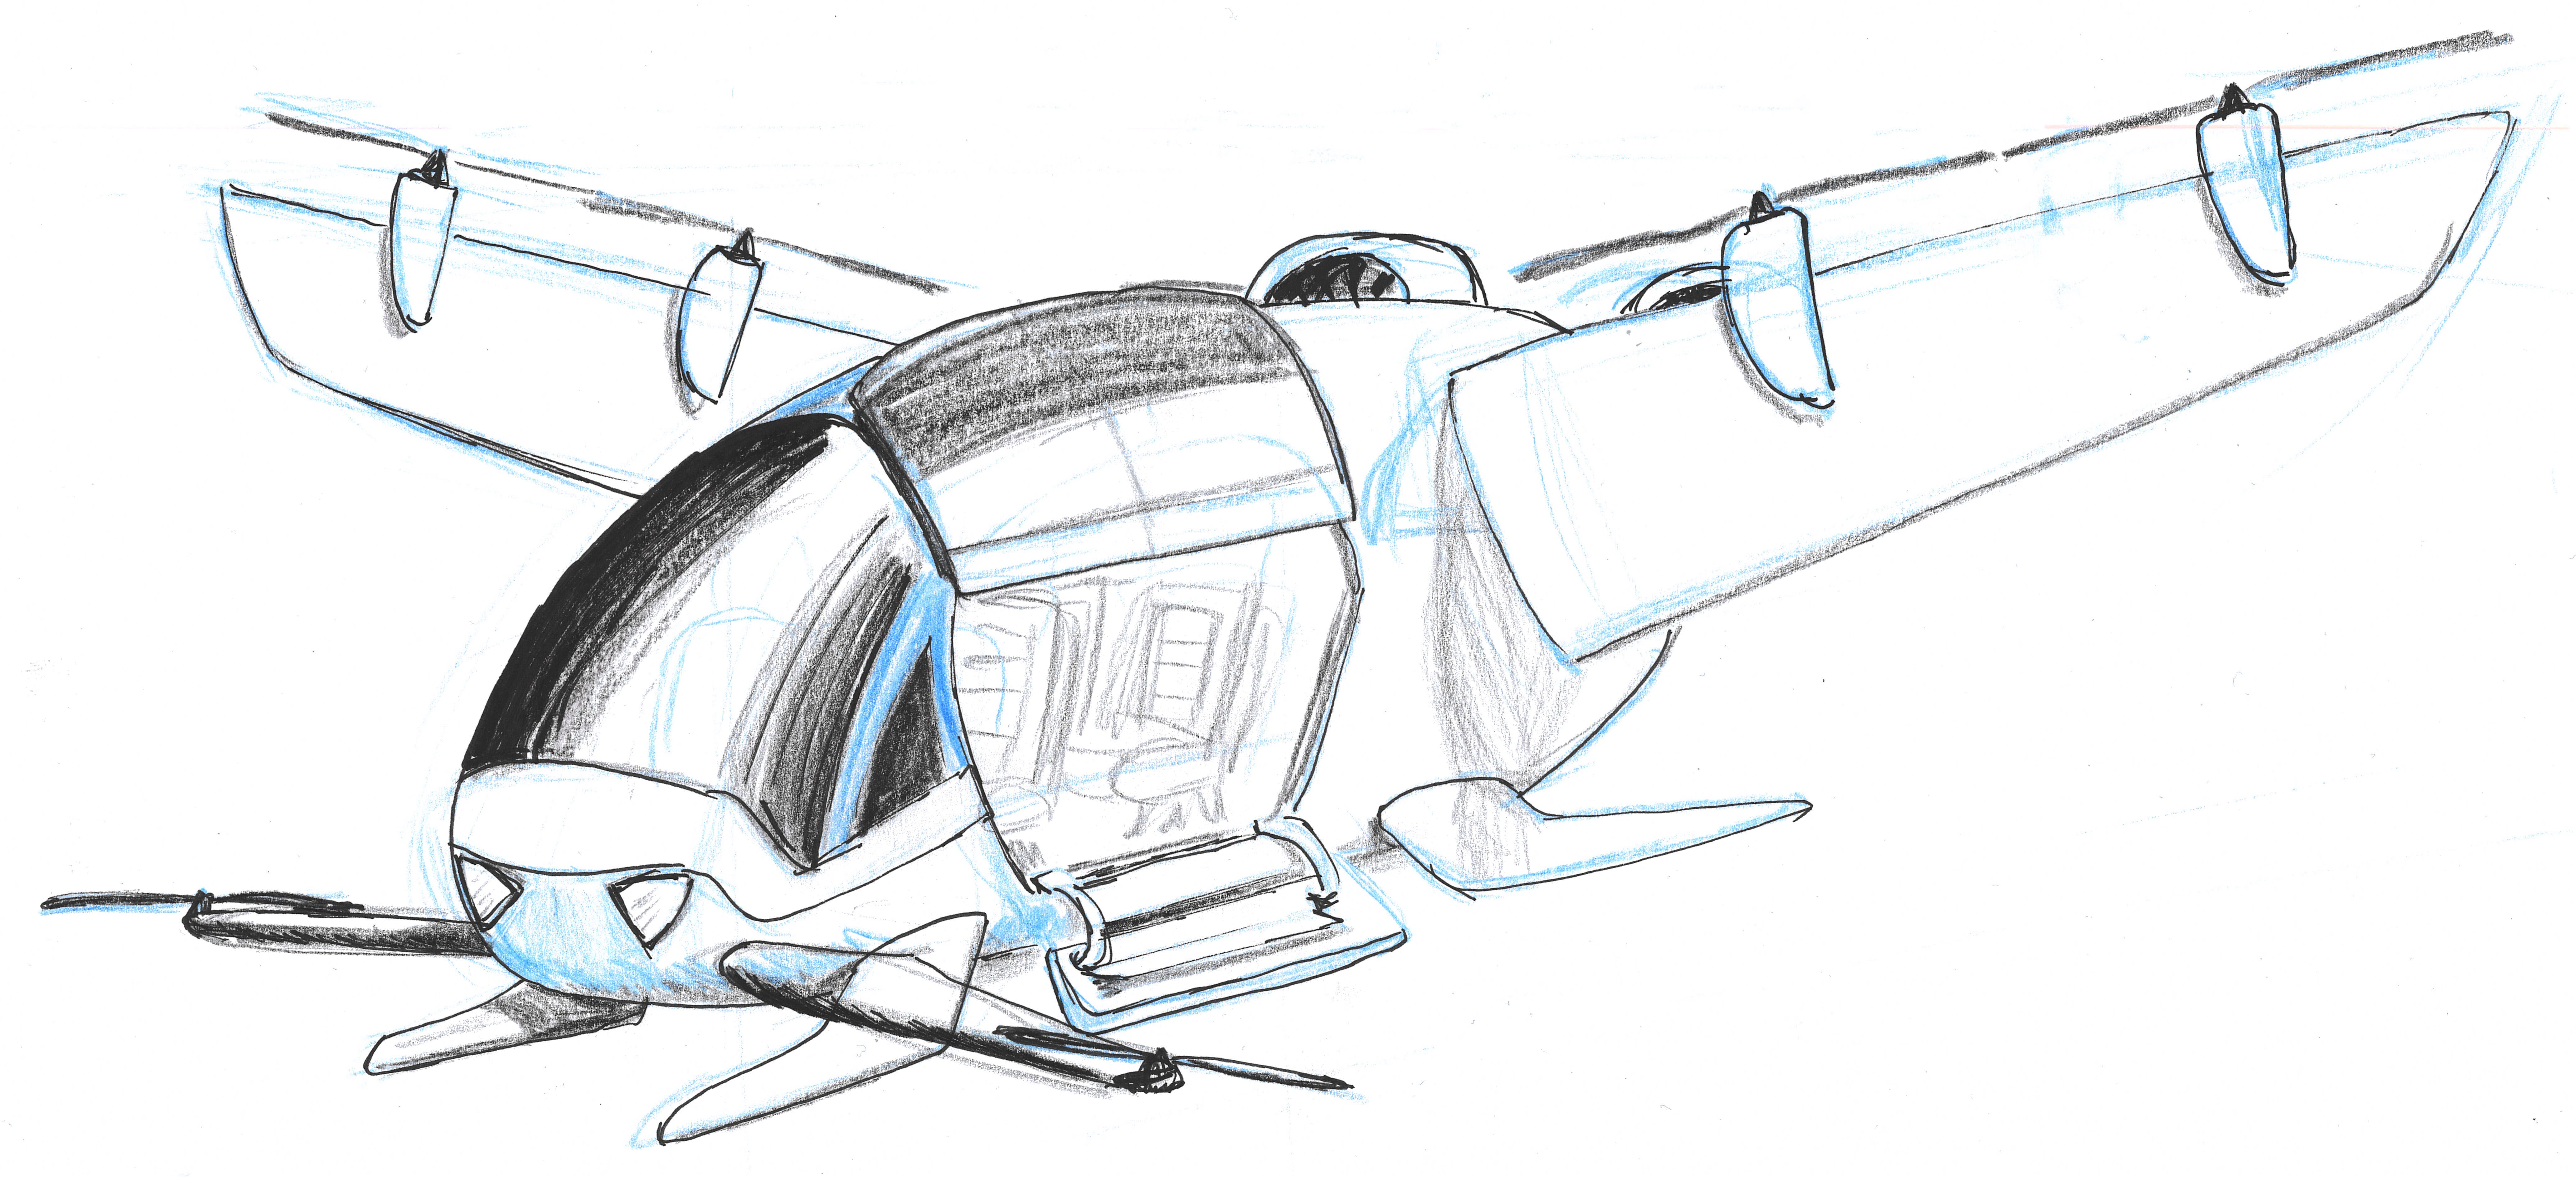
\includegraphics[width=5.0cm]{./Figures/bumblebee.jpg}
    \captionsetup{justification=centering}
    \caption{Tilt-wing 4}
    \label{4-6B}
  \end{minipage}
  \hspace{0.5cm}
  \begin{minipage}[b]{0.25\textwidth}
    \includegraphics[width=5.0cm]{./Figures/carriage.jpg}
    \captionsetup{justification=centering}
    \caption{Gondola 6}
    \label{4-6C}
  \end{minipage}  
\end{figure}


\begin{table}[H]
\captionsetup{justification=centering}
\caption{Input of tools for 4-6 person vehicle}
\label{46input}
\begin{tabular}{@{}llll@{}}
\toprule
\textbf{Parameter}                       & \textbf{Electric jet 4} & \textbf{Tilt-wing 4} & \textbf{Gondola 6} \\ \midrule
MTOW {[}kg{]}                            & 1339                   & 971                   & 2204                    \\
OEW/MTOW           & 0.35                   & 0.35                   & 0.35                    \\
\# Passengers {[}-{]}                    & 4                   &  4                  & 6                   \\
Range {[}km{]}                           & 54                   &  60                  & 45                    \\
Max Dimension {[}m{]}                    & 9                   & 10                    & 9                   \\
Battery Energy density {[}Wh/kg{]}       & 260                   & 260                    & 260                      \\
Battery Power density {[}W/kg{]}         & 2100                   & 2100                   &     2100                \\
L/D {[}-{]}                              & 17                   & 15                   & 4                    \\
Radius of rotors (x number of rotors)      & 0.15 (x36)           & 1 (x4); 1.5 (x1); 0.7 (x2) & 1.5 (x8)                    \\
Cruise Velocity {[}m/s{]}                & 60                   & 82                    & 34                    \\ \bottomrule
\end{tabular}

\end{table}


\subsection{Intermediate Trade-off}
%Present the outputs of the tools for each option, put it in a table and discuss which 1 (or 2) is best. Explain that we will continue with that one to the final trade off, where we will investigate that option further by looking at additional qualitative factors like user experience, passenger comfort, safety etc.. 
After designing the different vehicles a trade-off has been done to come up with the "best" vehicle. In \autoref{46output} the results for each design can be seen. The design process will continue with the Tilt-wing 4. This vehicle has the lowest energy usage, which makes it the most sustainable concept. Next to that, it has the lowest noise emission. If the pad costs are included in the ticket price, this vehicle is not the best option, due to the maximum dimension. However, if the pad costs will be excluded in the calculation for the ticket price it is the best solution. Therefore, the design process will continue with the Tilt-wing 4.


\begin{table}[H]
\captionsetup{justification=centering}
\caption{Output of tools for 4-6 person vehicle}
\label{46output}
\begin{tabular}{@{}llll@{}}
\toprule
\textbf{Parameter}                           & \textbf{Electric jet 4} & \textbf{Tilt-wing 4} & \textbf{Gondola 6} \\ \midrule
\# Vehicles {[}-{]}                          & 4000                   & 3350                   & 4730                   \\
\# Pads {[}-{]}                              & 840                   & 800                   & 880                    \\
\# Trips/day {[}-{]}                         & 131000                   & 124000               & 100000                   \\
\# PREE {[}Wh/(pax-km){]}                   & 1170                     & 670                    & 1510  \\
\# Ticket price {[}\$/km{]}                  & 3.35                   & 3.85                   & 3.25                    \\
\# Ticket price {[}\$/km-pad costs{]}        & 0.51                    & 0.42                   & 0.58                   \\
\# Passengers/day {[}-{]}                    & 281000                   & 269000                   & 316000                    \\
Vertiport Area {[}m\textsuperscript{2}{]}    & 1620                   & 2870                   & 1620                    \\
Total System Area {[}km\textsuperscript{2}{]}& 1.36                   & 1.55                   & 1.42                   \\
Total Board Time {[}s{]}                     & 300                    & 300                   & 390                   \\
rplNoise {[}dBA{]}                              & 110                   & 74                   & 90                    \\
Downwash {[}m/s{]}                              &             96       &     33          &          26        \\\bottomrule
\end{tabular}
\end{table}

\section{20+ Passenger Vehicles}
%Give a little introduction to 20+ passenger vehicles
Larger than 'car-sized' UAM vehicles are not often looked at in present studies. However, the team thinks that it's worth considering the class of 20 or more people. It has the potential advantages of having less vehicles and less landing sites, while carrying more people at once. Challenges will be the power and energy requirements that vehicles of this size will impose on the battery. The team came up with three concepts for this size, each of which will be evaluated with the aid of a tool. At the end of the section, one 'winner' will be selected to investigate further and compare to the best concepts for the other vehicle capacities. 

\subsection{Concept Definition}
Below, a sketch of each of the three concepts is given.  

\begin{figure}[H]
  \centering
  \begin{minipage}[b]{0.25\textwidth}
    \includegraphics[width=5.0cm]{./Figures/Concept_20A.png}
    \captionsetup{justification=centering}
    \caption{Concept 20A}
    \label{concept20a}
  \end{minipage}
  \hspace{1.25cm}
  \begin{minipage}[b]{0.25\textwidth}
    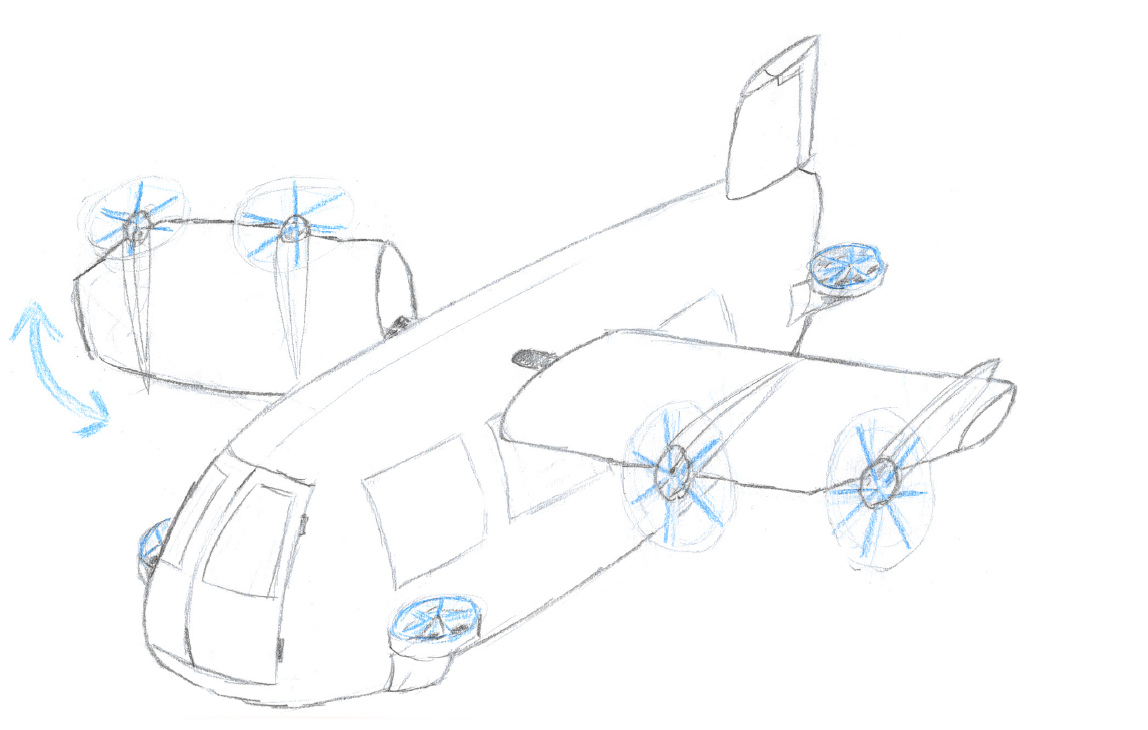
\includegraphics[width=5.0cm]{./Figures/Concept_20B.png}
    \captionsetup{justification=centering}
    \caption{Concept 20B}
    \label{concept20b}
  \end{minipage}
  \hspace{1.25cm}
  \begin{minipage}[b]{0.25\textwidth}
    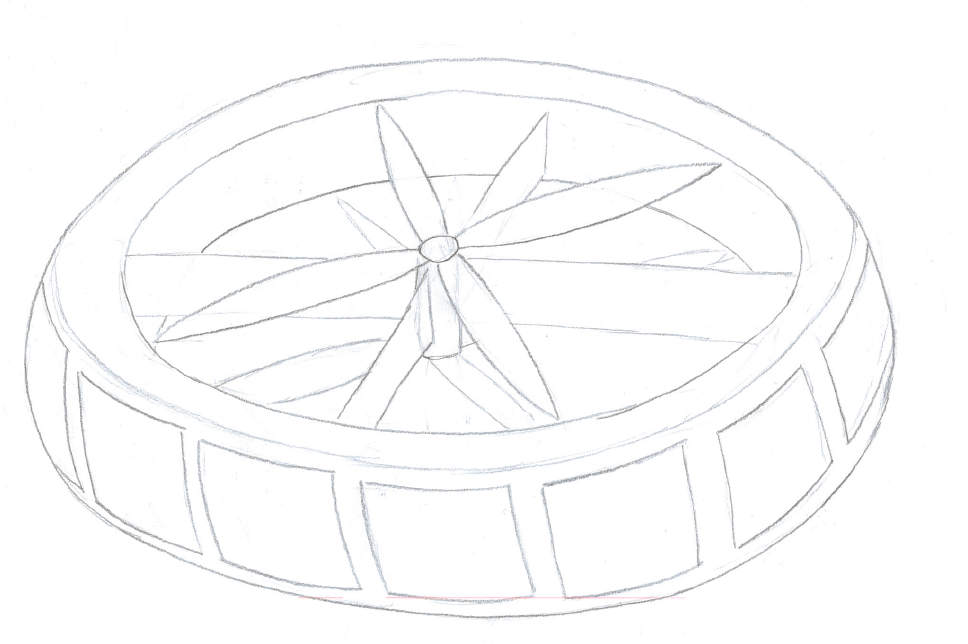
\includegraphics[width=5.0cm]{./Figures/Concept_20D.png}
    \captionsetup{justification=centering}
    \caption{Concept 20C}
    \label{concept20c}
  \end{minipage}  
\end{figure}

\paragraph{Concept 20A}
Concept 20A features both a fixed wing and tilting rotors. The passengers enter the vehicle through the back and sit in a 3 abreast configuration, with a total of 7 rows. At take-off the 4 propellers provide the thrust to lift off and, at a specified height, they will rotate to provide the thrust and part of the lift in cruise. The vehicle will land on a set of wheels in tricycle configuration and can then be plugged in for charging. The battery of the vehicle will be under the floor of the passengers. More details on this vehicle concept can be found in \autoref{20input}.  

\paragraph{Concept 20B}
Concept 20B is a tilt wing concept. The passengers enter through the front of the aircraft and sit 4 abreast in a one-aisle configuration. There will be 5 rows to accommodate 20 passengers. It features 4 rotors on the wings and 2 on the back and front respectively to provide stability, resulting in a total of 8 rotors. All of these rotors will be used at take-off, landing and hover. For the cruise phase the wings will tilt such that the propellers provide the thrust, the wings will provide all the lift needed for flight. The smaller rotors at the front and rear of the aircraft will be predominantly used for the longitudinal stability. The landing gear and battery will, as in concept 1, be located under the the floor of the passengers. Extra room for batteries is available in the back. More details on this vehicle concept can be found in \autoref{20input}.  

\paragraph{Concept 20C}
Concept 20C is a design that is quite different to the ones seen so far. It's a coaxial rotor surrounded by a passenger compartment. The passengers will be seated in a circle configuration around this rotor facing outwards. The large rotor will provide the lift, thrust and stability. The battery will be located under the floor and in the structure that holds the rotor in place. The latter will cause a bending relief.  Again, more details on this vehicle concept can be found in \autoref{20input}.  

The three options are summarised in table \autoref{20input}. They will be inputted in the tool with the goal of comparing the different concepts in this vehicle class at a later stage. 

\begin{table}[H]
\captionsetup{justification=centering}
\caption{Input of tools for 20+ person vehicle}
\label{20input}
\begin{tabular}{@{}llll@{}}
\toprule
\textbf{Parameter}                       & \textbf{Concept 20A} & \textbf{Concept 20B} & \textbf{Concept 20C} \\ \midrule
MTOW {[}kg{]}                            &    9000                &       7000             &  12000                  \\
OEW/MTOW           &        45            &           45         &      40              \\
\# Passengers {[}-{]}                    &        21            &        20            &       20             \\
Range {[}km{]}                           &        60            &        60            &           20         \\
Max Dimension {[}m{]}                    &          18         &        18            &          16          \\
Battery Energy density {[}Wh/kg{]}       &         260            &     260               &       250             \\
Battery Power density {[}W/kg{]}         &           2100        &        2100            &         2500           \\
L/D {[}-{]}                              &         8.0           &        13            &     2               \\
Radius of rotors (x number of rotors)  &           2.5 (x4)         &   1.85 (x4), 0.85 (x4)                 &     6 (1x)               \\
Cruise Velocity {[}m/s{]}                &          83          &        111           &  42                 \\ \bottomrule
\end{tabular}

\end{table}


\subsection{Intermediate Trade-off}
%Present the outputs of the tools for each option, put it in a table and discuss which 1 (or 2) is best. Explain that we will continue with that one to the final trade off, where we will investigate that option further by looking at additional qualitative factors like user experience, passenger comfort, safety etc.. 

As mentioned before, the inputs that were specified in the previous section are fed through a tool that computes some outputs that will be the basis for comparing the concepts in this vehicle class.  


\begin{table}[H]
\captionsetup{justification=centering}
\caption{Output of tools for 20+ person vehicle}
\label{20output}
\begin{tabular}{@{}llll@{}}
\toprule
\textbf{Parameter}                           & \textbf{Concept 20A} & \textbf{Concept 20B} & \textbf{Concept 20C} \\ \midrule
\# Vehicles {[}-{]}                          &       1600             &     1500            &      1700                 \\
\# Pads {[}-{]}                              &         570           &      550           &          645            \\
\# Trips/day {[}-{]}                         &         25800           &       26000          &         20000               \\
\#  PREE {[}Wh/(pax-km){]}           &        1690           &       1230         &         5160            \\
\# Ticket price per kilometre {[}\$/(km){]} &           7.81           &          7.84       &        13.70               \\
\# Ticket price {[}\$/km-pad costs{]}        & 0.63                    &      0.59            &   --            \\
\# Passengers/day {[}-{]}                    &         268000           &       259000          &      209000               \\
Vertiport Area {[}m\textsuperscript{2}{]}    &           5700         &        5700         &        4600              \\
Total System Area {[}km\textsuperscript{2}{]} &       3.23             &      3.12           &       2.94               \\
Total Board Time {[}s{]}                     & 1065                   &     1020            &      1020                \\
Noise {[}dBA{]}                              &           90        &      90           &       94                  \\
Downwash {[}m/s{]}                              &             45       &     48          &  --   \\ \bottomrule
\end{tabular}

\end{table}

From the table it is clear that concept 20B is the best to proceed with. The energy usage per passenger kilometre and the ticket price per kilometre for concept 3 are too high to high to continue with this one. Comparing concept 20A and 20B, it can be seen that concept 20B has a energy usage per passenger kilometre that is significantly higher. This is mostly due to the more aerodynamic shape and the larger wing, that follow in a higher estimation for the $L/D$. Furthermore, the noise of option 20B is somewhat lower. All in all concept 20B seems like the best option to continue with. This option will be investigated further in \autoref{Sec:FinalTO}.  




\section{Final Trade-off}
\label{Sec:FinalTO}
%Present qualitative aspects for each final concept
%run the final trade off
%present the final 
Now that the most feasible options for each vehicle passenger range have been selected, it is time to compare them to each other. For clarity an overview of the inputs and outputs for the winning concepts in each category are shown below in \autoref{inputswin}. 

\begin{table}[H]
\captionsetup{justification=centering}
\caption{Inputs of winning vehicles}
\label{inputswin}
\begin{tabular}{llll}
\hline
\textbf{Parameter}                    & \textbf{1-2 pax}      & \textbf{4-6 pax} & \textbf{20+ pax}    \\ \hline
MTOW {[}kg{]}                         & 575                   &    971              & 7418                \\
OEW/MTOW        & 0.40                    &   0.35          & 0.45                  \\
\# Passengers {[}-{]}                 & 2                     &      4            & 20                  \\
Range {[}km{]}                        & 60                    &                  & 60                  \\
Max Dimension {[}m{]}                 & 5                     &                  & 18                  \\
Battery Energy density {[}Wh/kg{]}    & 260                &                  & 260               \\
Battery Power density {[}W/kg{]}      & 2100               &                  & 2100              \\
L/D {[}-{]}                           & 12                    &                  & 13                  \\
Radius of rotors (x number of rotors) & 0.85 (2x) \& 0.8 (2x) &                  & 2.5 (x4), 0.85 (x4) \\
Cruise Velocity {[}m/s{]}             & 32                    &                  & 111.1               \\ \hline
\end{tabular}
\end{table}

\begin{table}[H]
\captionsetup{justification=centering}
\caption{Outputs of winning vehicles}
\label{outputswin}
\begin{tabular}{llll}
\hline
\textbf{Parameter}                          & \textbf{1-2 pax} & \textbf{4-6 pax} & \textbf{20+ pax} \\ \hline
\# Vehicles {[}-{]}                         & 12900             &                  & 1230             \\
\# Pads {[}-{]}                             & 1620             &                  & 491              \\
\# Trips/day {[}-{]}                        & 308000           &                  & 19298            \\
\# PREE {[}Wh/(pax-km){]}                   & 790           &                  & 1406.0           \\
\# Ticket price per kilometre {[}\$/(km){]} & 4.12             &                  & 9.36             \\
\# Passengers/day {[}-{]}                   & 32700           &                  & 202758           \\
Vertiport Area {[}m\textsuperscript{2}{]}   & 630            &                  & 5699             \\
Total System Area {[}km\textsuperscript{2}  & 1.48          &                  & 2793200          \\
Total Board Time {[}s{]}                    & 210              &                  & 1020             \\
Noise {[}dBA{]}                             & 71             &                  & 84.5             \\ \hline
\end{tabular}
\end{table}


NEED TO UPDATE THIS!!!!!!!!!!!!!!!!!!!!!!!!!!!!!!!!!!!!!!!!!!!!!!!!!!!!!!!!!!!!!!

Naturally, this list of quantitative parameters is not the complete picture. There are other factors of a potential UAM system that are of relevance too. They are the ones that are of qualitative nature and have therefore not been examined in the tool. The factors that are looked at are the safety, the passenger experience, the ATM/UTM efforts needed, the susceptibility to harsh weather conditions and the modifications that would have to be done to the current regulations for a system to work. Each of these five factors will be given a score in the range from 1-5 and, after which this number is multiplied with the weight that was assigned to it in \autoref{subsec:weights}. A weighted average is computed for each of the concepts. All of the aforementioned can be found in table (REF TO TABLE) below. 

%THE ULTIMATE TABLE!!!!! THIS INCLUDES OUR CRITERIA WITH THEIR WEIGHTS AND THE SCORE THAT THEY GET. INCLUDE A WEIGHTED AVERAGE FOR EACH OF THE CONCEPTS AND THERE WE HAVE IT: ---> OUR WINNING CONCEPT <--- 





As can be seen from the table concept XXX is the winner. This will be the concept that will be further worked out in the final phase of the project. 


